\chapter{DESENVOLVIMENTO}

\section{Diodo Zener - Modelo Simplificado}

\begin{figure}[H]
    \centering
    \fbox{
        \parbox{0.975\textwidth}{
            \centering
            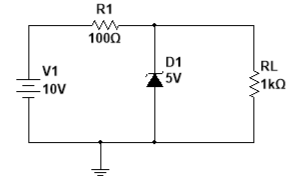
\includegraphics[]{images/imagem_slide_01.png}
        }}
    \caption{Circuito 01}
    \vspace{-0.3cm}
    \label{fig:Circuito01}
\end{figure}

Para a primeira avaliação substituiremos o Diodo Zener (Imagem \ref{fig:Circuito01}) por uma fonte de tensão de 5v, o circuito com a modificação é mostrado na Imagem \ref{fig:Circuito02}.

\begin{figure}[H]
    \centering
    \fbox{
        \parbox{0.975\textwidth}{
            \centering
            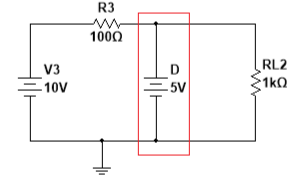
\includegraphics[]{images/circuito_01_substituido.png}
        }}
    \caption{Circuito 01 - Com substituição do Zener por fonte}
    \vspace{-0.3cm}
    \label{fig:Circuito01ComSubstituicao}
\end{figure}

Considerando o circuito da figura \ref{fig:Circuito01ComSubstituicao}, temos que:

\begin{Resolucao}[H]
    \fbox{
        \parbox{0.975\textwidth}{
            \vspace{0.40cm}
            \centering
            \[V0 = Vz = \textcolor{red}{5V}\]
            \[IRL = \frac{Vz}{Rl} \rightarrow \frac{5V}{1K} = \textcolor{red}{5mA}\]
            \[It = \frac{Vi - Vz}{Rs} \rightarrow \frac{10 - 5}{1K} = \textcolor{red}{50mA}\]
            \[Iz = It - Irl \rightarrow 50mA - 5mA = \textcolor{red}{45mA}\]
        }
    }
    \captionof*{Resolucao}{Resolução: Circuito Exercício 1}
    \label{res:circuito01}
\end{Resolucao}

\begin{figure}[H]
    \centering
    \fbox{
        \parbox{0.975\textwidth}{
            \centering
            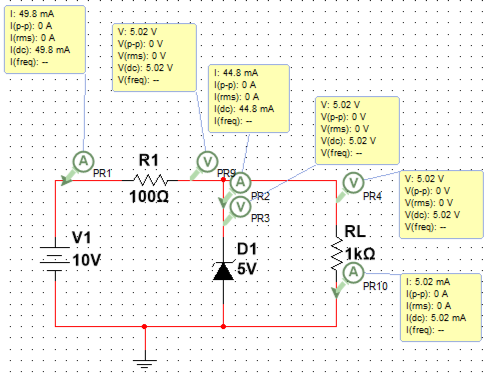
\includegraphics[]{images/simulacoes/circuito01.png}
        }}
    \caption{Simulação: Circuito 01}
    \vspace{-0.3cm}
    \label{fig:SimulacaoCircuito01}
\end{figure}

Com a tabela \ref{tab:Comparacao1Circuito} podemos comparar os resultados obtidos por simulação com os resultados obtidos por cálculo, na qual comprovam que os cálculos estavam corretos.

\begin{quadro}[H]
    \centering
    \caption{Comparação entre os resultados obtidos por simulação e os resultados obtidos por cálculo do circuito 01}
    \begin{tabular}{|C{0.19\textwidth}|C{0.15\textwidth}|C{0.15\textwidth}|C{0.15\textwidth}|C{0.15\textwidth}|}
        \hline
        \rowcolor[HTML]{C0C0C0}
        \textbf{Modelo\textbackslash{}Variáveis} & \textbf{Vo} & \textbf{IRL} & \textbf{It} & \textbf{Iz} \\
        \hline
        Calculado & 5V & 5mA & 50mA & 45mA \\
        \hline
        Simulado & 5.02V & 5.02mA & 49.98mA & 44.8mA \\
        \hline
    \end{tabular}
    \vspace{-0.6cm}
    \label{tab:Comparacao1Circuito}
\end{quadro}

\subsection{Circuito 1 com fonte de tensão em 12V}

Observamos que como Vo é igual a tensão no resistor, a saída do circuito é constante ditada pelo diodo Zener, neste caso se aumentarmos a tensão da fonte teremos uma corrente maior circulando pelo circuito logo temos:

\begin{Resolucao}[H]
    \fbox{
        \parbox{0.975\textwidth}{
            \vspace{0.40cm}
            \centering
            \[It = \frac{Vi - Vz}{RS} \rightarrow \frac{12 - 5}{100} = \textcolor{red}{70mA}\]
            \[Iz = It - Irl \rightarrow 70mA - 5mA = \textcolor{red}{65mA}\]
        }
    }
    \captionof*{Resolucao}{Resolução: Circuito Exercício 2}
    \label{res:circuito02}
\end{Resolucao}

Podemos observar que não há variação na saída ao alterarmos a tensão de entrada do circuito, a tensão na carga permanece constante devido à atuação do diodo Zener no modelo simplificado.

\section{Regulador Zener de Modelo Linear}

\subsection{Fonte em 10V}

\begin{figure}[H]
    \centering
    \fbox{
        \parbox{0.975\textwidth}{
            \centering
            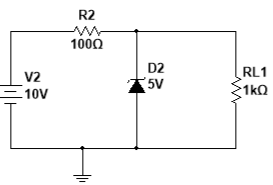
\includegraphics[]{images/imagem_slide_02.png}
        }}
    \caption{Circuito 02}
    \vspace{-0.3cm}
    \label{fig:Circuito02}
\end{figure}

Para a primeira avaliação substituiremos o Diodo Zener (Imagem \ref{fig:Circuito02}) por uma fonte de tensão de 5v seguido de uma resistência de 100$\Omega$, o circuito com a modificação é mostrado na Imagem \ref{fig:Circuito02}.

\begin{figure}[H]
    \centering
    \fbox{
        \parbox{0.975\textwidth}{
            \centering
            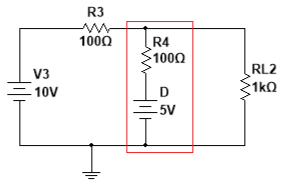
\includegraphics[]{images/circuito_02_substituido.png}
        }}
    \caption{Circuito 02 - Com substituição do Zener por fonte e resistor}
    \vspace{-0.3cm}
    \label{fig:Circuito02}
\end{figure}

Considerando o modelo Linear, o diodo possui uma faixa de atuação sendo uma corrente máxima de operação, se o diodo ultrapassar essa corrente máxima ele vai queimar e uma corrente mínima no qual será 10\% da corrente máxima que o diodo suporta, o comportamento é mostrado na imagem \ref{fig:comportamentoZener}.

\begin{figure}[H]
    \centering
    \fbox{
        \parbox{0.975\textwidth}{
            \centering
            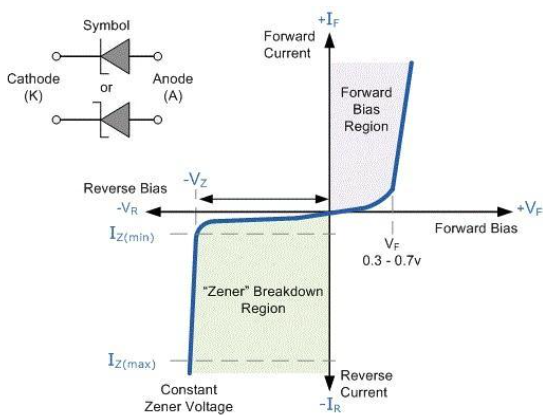
\includegraphics[]{images/comportamento_diodo_zener.png}
        }}
    \caption{Comportamento de um diodo Zener}
    \vspace{-0.3cm}
    \label{fig:comportamentoZener}
\end{figure}

Quando a operação do diodo Zener está no quadrante acima e a direita ele está polarizado diretamente e seu funcionamento é igual ao de um diodo comum. No estado quando está polarizado diretamente ele opera com uma tensão constante teoricamente. A região entre as correntes IzMin e IzMax é a área de operação do diodo Zener.

\begin{Resolucao}[H]
    \fbox{
        \parbox{0.975\textwidth}{
            \centering
            \[Vi = 10V\]
            \[Rl = 1K\Omega\]
            \[RS = 100\Omega\]
            \[RZ = 7\Omega\]
            \[Vz = 5.1V\]
            \[Vz0 = 4.85V\]
            \[Izt = 49mA\]
        }
    }
    \captionof*{Resolucao}{Dados: Circuito Exercício 3}
    \label{res:circuito03}
\end{Resolucao}

Considerando os dados acima, os cálculos ficam em:

\begin{Resolucao}[H]
    \fbox{
        \parbox{0.975\textwidth}{
            \centering
            \[It = Iz + IRL\]
            \[It = \frac{Vi - Vz}{RS} = \frac{Vz - Vz0}{RZ} + \frac{Vz}{RL}\]
            \[It = \frac{10 - Vz}{100} = \frac{Vz - 4.85}{7} + \frac{Vz}{1000}\]
            Se aplicando MMC:
            \[\frac{10 - Vz}{100} = \frac{Vz - 4.85}{7} + \frac{Vz}{1000} \]
            \dots\[\frac{700 - 70Vz}{7000} = \frac{1000Vz - 4850}{7000} + \frac{7Vz}{7000}\]
            \[1000Vz + 7Vz + 70Vz = 700 + 4850\]
            \[1077Vz = 5550 \rightarrow Vz = \frac{5550}{1077}\]
            \[Vz1 = \textcolor{red}{5.15V}\]
        }
    }
    \captionof*{Resolucao}{Resolução: Circuito Exercício 3 - Fonte em 10V}
    \label{res:circuito03}
\end{Resolucao}

\begin{figure}[H]
    \centering
    \fbox{
        \parbox{0.975\textwidth}{
            \centering
            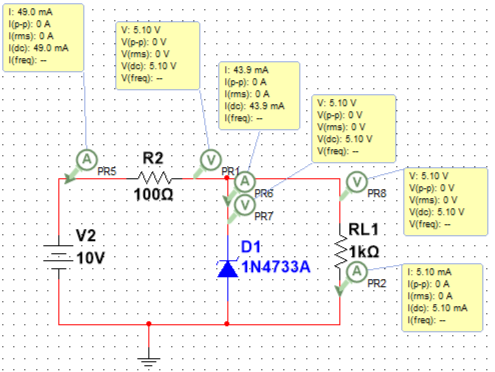
\includegraphics[]{images/simulacoes/circuito02.png}
        }}
    \caption{Simulação: Circuito 02 - Com fonte de 10V}
    \vspace{-0.3cm}
    \label{fig:SimulacaoCircuito03}
\end{figure}

\subsection{Fonte em 12V}

\begin{Resolucao}[H]
    \fbox{
        \parbox{0.975\textwidth}{
            \centering
            \[It = Iz + IRL\]
            \[It = \frac{Vi - Vz}{RS} = \frac{Vz - Vz0}{RZ} + \frac{Vz}{RL}\]
            \[It = \frac{12 - Vz}{100} = \frac{Vz - 4.85}{7} + \frac{Vz}{1000}\]
            Se aplicando MMC:
            \[\frac{12 - Vz}{100} = \frac{Vz - 4.85}{7} + \frac{Vz}{1000} \rightarrow \frac{840 - 70Vz}{7000}\]
            \dots\[\frac{1000Vz - 4850}{7000} + \frac{7Vz}{7000}\]
            \[840 - 70Vz = 1000Vz - 4850 + 7Vz\]
            \[1000Vz + 7Vz + 70Vz = 840 + 4850\]
            \[1077Vz = 5690 \rightarrow Vz = \frac{5690}{1077}\]
            \[Vz2 = \textcolor{red}{5.28V}\]
        }
    }
    \captionof*{Resolucao}{Resolução: Circuito Exercício 3 - Fonte em 12V}
    \label{res:circuito04}
\end{Resolucao}

\begin{figure}[H]
    \centering
    \fbox{
        \parbox{0.975\textwidth}{
            \centering
            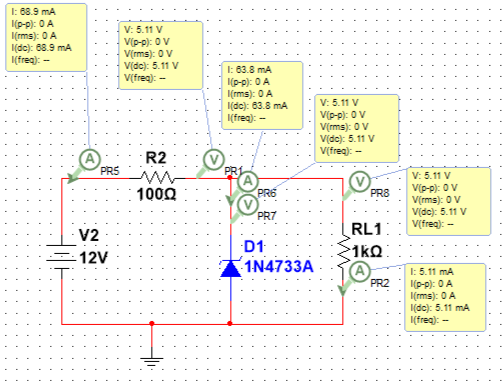
\includegraphics[]{images/simulacoes/circuito03.png}
        }}
    \caption{Simulação: Circuito 02 - Com fonte em 12V}
    \vspace{-0.3cm}
    \label{fig:SimulacaoCircuito04}
\end{figure}

Com a tabela \ref{tab:ComparacaoCircuito02Com10V} podemos comparar os resultados obtidos por simulação com os resultados obtidos por cálculo com fonte de tensão em 10V, na qual comprovam que os cálculos estavam corretos.

\begin{quadro}[H]
    \centering
    \caption{Comparação entre os resultados obtidos por simulação e os resultados obtidos por cálculo do circuito 02 - 10V}
    \begin{tabular}{|C{0.19\textwidth}|C{0.13\textwidth}|C{0.13\textwidth}|C{0.13\textwidth}|C{0.13\textwidth}|C{0.13\textwidth}|}
        \hline
        \rowcolor[HTML]{C0C0C0}
        \textbf{Modelo\textbackslash{}Variáveis} & \textbf{Vo} & \textbf{IRL} & \textbf{It} & \textbf{Iz} & \textbf{Vz} \\
        \hline
        Teórico & 5V & 5mA & 50mA & 45mA & 5.15V \\
        \hline
        Simulado & 5.02V & 5.02mA & 49.8mA & 44.8mA & 5.10V \\
        \hline
    \end{tabular}
    \vspace{-0.6cm}
    \label{tab:ComparacaoCircuito02Com10V}
\end{quadro}

Com a tabela \ref{tab:ComparacaoCircuito02Com12V} podemos comparar os resultados obtidos por simulação com os resultados obtidos por cálculo com fonte de tensão em 12V, na qual comprovam que os cálculos estavam corretos.

\begin{quadro}[H]
    \centering
    \caption{Comparação entre os resultados obtidos por simulação e os resultados obtidos por cálculo do circuito 02 - 12V}
    \begin{tabular}{|C{0.19\textwidth}|C{0.13\textwidth}|C{0.13\textwidth}|C{0.13\textwidth}|C{0.13\textwidth}|C{0.13\textwidth}|}
        \hline
        \rowcolor[HTML]{C0C0C0}
        \textbf{Modelo\textbackslash{}Variáveis} & \textbf{Vo} & \textbf{IRL} & \textbf{It} & \textbf{Iz} & \textbf{Vz} \\
        \hline
        Teórico & 5V & 5mA & 70mA & 65mA & 5.28V \\
        \hline
        Simulado & 5.02V & 5.02mA & 69.8mA & 64.7mA & 5.11V \\
        \hline
    \end{tabular}
    \vspace{-0.6cm}
    \label{tab:ComparacaoCircuito02Com12V}
\end{quadro}

Caso seja feita regulação com variação de 20\%:

\begin{Resolucao}[H]
    \fbox{
        \parbox{0.975\textwidth}{
            \centering
            \[\frac{Vz2 - Vz1}{Vz1} \rightarrow \frac{5.28 - 5.15}{5.15} * 100 = \textcolor{red}{2.52\%}\]
        }
    }
    \captionof*{Resolucao}{Regulação: 20\% sobre o valor nominal}
    \label{res:circuito05}
\end{Resolucao}